\section{swf,影音,附件宏包}
\subsection{animate 宏包}

\index{命令!\verb$\animategraphics$}
\index{宏包!animate}
\begin{lstlisting}
\usepackage[`可选项`]{animate}
\animategraphics{12}{frames}{}{} `默认全部播放`
\animategraphics[`可选项`]{`速率`}{`文档名`}{`起始页码`}{`结束页码`}
\end{lstlisting}

参数中主要的选项有:controls,loop, 实现显示控制按钮和自动循环。

\begin{figure}[htbp]%位置选项
\centering
\animategraphics[controls,loop]{10}{body/_fig0020}{}{}\\
\caption{动画图片} \label{mov}
\end{figure}


\subsection{MOV15 宏包}

\index{命令!\verb$\includemovie$}
\index{宏包!mov15}
\color{red}
注意:MOV15是直接嵌入 PDF 中观看,attachfile 是双击后在外部观看$\checkmark $。\\
\normalcolor
相关代码如下:
\begin{shaded}
\begin{Verbatim}
\usepackage[<package options>]{movie15}%可选项3D
\includemovie[<options>]{<width>}{<height>}{<media file>}
\includemovie[autostop,controls,
text={\textcolor{blue}{点击播放!}}]
{10cm}{10cm}{clock.avi}\\
\end{Verbatim}
\end{shaded}


可选项中选 autostop,controls,和 text={},会出现进度条和首次看的页面。
%\begin{figure}[H]
%\centering
%\includemovie[text={\textcolor{blue}{点击播放!}},controls,autostop]%
%{10cm}{10cm}{clock.avi}\\
%~\\
%  \caption{movie15 影音播放}\label{movie}
%\end{figure}

支持的格式有如\ref{movie15}所示\\
\begin{table}[ht]
  \centering
   \caption{movie15 宏包支持格式}\label{movie15}
  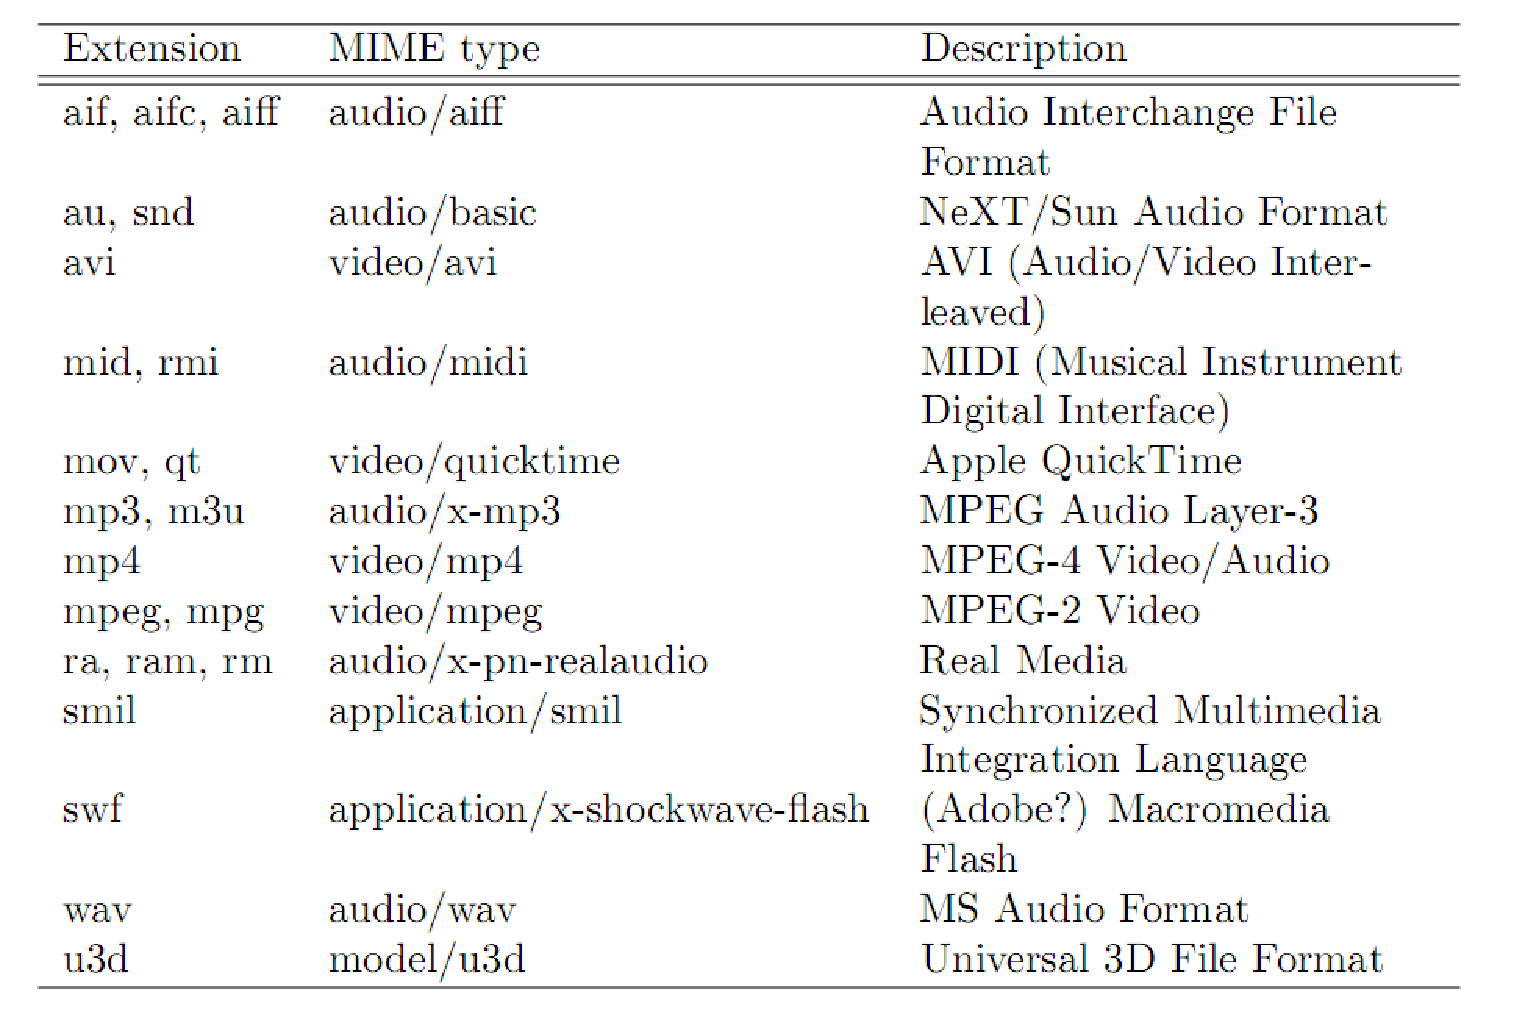
\includegraphics[width=14cm]{movie_format}\\

\end{table}

\subsection{attachfile2 宏包}

\index{命令!\verb$\textattachfile$}
\index{宏包!attachfile}
如\ref{movie_attach}所示双击在新文件中打开,注意如果在福昕阅读器中,
文件放在子文件夹内会读不出来反斜杠 \textcolor[rgb]{1.00,0.00,0.00}{/} 字符而不能播放,
AdobeReder 则没有问题,另外如果双击后无法打开 swf 文件,可能是播放器没有关联 swf 文件,可用 kmplayer 关联 swf 格式。
 \begin{shaded}
 \begin{Verbatim}
 \textattachfile{文件名}
 {\includegraphics[width=10cm]{封面}}
 \end{Verbatim}
 \end{shaded}

\begin{figure}[ht]
  \centering
\textattachfile{vim.swf}{
\includegraphics[width=10cm]{VIM.pdf}} \\
 \caption{attachfile 视频播放}\label{movie_attach}
\end{figure}
~\\


\begin{cmd}[label=attachfile2 使用样例代码]
\hyperlink{symbols}{\color{blue}\uline{\LaTeX 常用符号}}
\hypertarget{symbols}{\textcolor[rgb]
{0.00,0.00,1.00}{双击下面图标打开文档}}
\normalcolor
~\\[0.3cm]
\begin{center}
\fbox{
\textattachfile{appendix/symbols.pdf} %这里加入所添加的附件
{\parbox[b][4cm][c]{3cm}{ \color{blue} symbols \\\LaTeX 常用符号}}
}
\end{center}
\end{cmd}
%
%效果见下一页:
%\hyperlink{symbols}{\color{blue}\uline{\LaTeX 常用符号}}
%\clearpage
%\hypertarget{symbols}{\textcolor[rgb]
%{0.00,0.00,1.00}{双击下面图标打开文档}}
%
%\begin{center}
%\fbox{
%\textattachfile{symbols.pdf} %这里加入所添加的附件
%{\parbox[b][4cm][c]{3cm}{ \color{blue} symbols \\\LaTeX 常用符号}}
%}
%\end{center}

\textcolor[rgb]{1.00,0.00,0.00}{注意:
attachfile2 支持 xelatex 模式,但不支持子文件夹,并与 hyperref 中选项有冲突,在导言区不能加入hyperref的 pdfauthor 等属性。}
